%%%%%%%%%%%%%%%%%%%%%%%%%%%%%%%%%%%%%%%%%%%%%%%%%%%%%%%%%%%%%%%%%%%%%%
% 调用ShanghaiTechThesis.cls文档声明
\documentclass[doctor,spst]{ShanghaiTechThesis}
    % 本科生使用 bachelor,硕士使用 master,博士使用 doctor
    % 物质学院用 spst,生命学院用 slst,信息学院用 sist
    % 以上两个选项必须各选一,否则会报错,具体代码见ShanghaiTechThesis.cls文档代码
%%%%%%%%%%%%%%%%%%%%%%%%%%%%%%%%%%%%%%%%%%%%%%%%%%%%%%%%%%%%%%%%%%%%%%
%导言区
    \classification{分类号}           
    \confidential{密级}             
    \UDC{UDC}                     
    \IDnumber{学号}               
    \cntitle{上海科技大学学位论文\LaTeX 模板示例文档}                
    %\scntitle{中文标题过长时启用}            
    \entitle{A Sample Document for \LaTeX-basedd }                   
    \sentitle{ShanghaiTech University Thesis Template}       %标题过长换行部分      
    \cnauthor{作\quad 者}                  
    \enauthor{Author}                  
    \cnadvisor{导\quad 师}                  
    \enadvisor{Advisor}                
    \cnresearch{研究方向}                
    \enresearch{research}               
    \cnmajor{二级专业}                    
    \enmajor{major}                   
    \cnsubmitdate{2000年1月1日}              
    \ensubmitdate{Jan. 1st, 2000}    
    %未启用           
    %\jobbegin{}
    %\jobend{} 
    %\reportfinish{} 
%%%%%%%%%%%%%%%%%%%%%%%%%%%%%%%%%%%%%%%%%%%%%%%%%%%%%%%%%%%%%%%%%%%%%%
\begin{document}
\maketitle\makeentitle            % maketitle 后面插入各种说明文档,不计入目录,用于插入各种说明性文档
                                  % 标题页的编写最好在cls文件中,当然也可以 include
    \cleardoublepage
	\thispagestyle{empty}
	\begin{center}
		{\bfseries\zihao{3} 上海科技大学学位论文原创性声明}
	\end{center}
	\vskip 10pt
	{\par\zihao{-4}本人郑重声明:所呈交的学位论文,是本人在导师的指导下, 
	独立进行研究工作所取得的成果。除文中已经注明引用的内容外,本论文不包含
	任何其他个人或集体已经发表或撰写过的作品成果。对本文的研究做出重要贡献
	的个人和集体,均已在文中以明确方式标明。本人完全意识到本声明的法律结果
	由本人承担。\par}
	\vskip 60pt
	\hspace{13em}学位论文作者签名:\hrulefill\hspace{1.5em}
	\vskip 15pt
	\hspace{16em}日\hspace{1em}期:\hrulefill\hrulefill 年 \hrulefill 月 \hrulefill 日\hspace{1em}

           % 原创性声明
    \cleardoublepage
	\pagestyle{empty}
	\begin{center}
	{\bfseries\zihao{3} 上海科技大学学位论文版权使用授权书}
	\end{center}
	\vskip 10pt
	{\par\zihao{-4}本学位论文作者完全了解学校有关保留、使用学位论文的规定,
	同意学校保留并向国家有关部门或机构送交论文的复印件和电子版,
	允许论文被查阅和借阅。本人授权上海交通大学可以将本学位论文的全部或部分内容
	编入有关数据库进行检索,可以采用影印、缩印或扫描等复制手段保存和汇编本学位论文。\par
	本学位论文属于\\
	\hspace*{9em}\textbf{保\hspace{1em}密} \rule{3mm}{3mm},
	在~\hrulefill~年解密后适用本授权书。\\
	\hspace*{9em}\textbf{不保密} \rule{3mm}{3mm} 。\\
	(请在以上方框上打勾)
	\par}
	\vskip 60pt
	学位论文作者签名:\hrulefill\hspace{3em}指导教师签名:\hrulefill
	\vskip 15pt
	日\hspace{1em}期:\hrulefill\hrulefill 年 \hrulefill 月 \hrulefill 日
	\hfill \hspace{3em}日\hspace{1em}期:\hrulefill\hrulefill 年 \hrulefill 月 \hrulefill 日      % 授权声明

\frontmatter\pagestyle{main}      % frontmatter 后 include 的 separatepage 开始有页码且页码为罗马数字
    \newcommand\cnkeywords[1]{\vspace{2ex}\noindent{\heiti 关键词:} #1}
\newcommand\enkeywords[1]{\vspace{2ex}\noindent{\bfseries Keywords:~} #1}


\chapter{摘\quad 要}
上海科技大学(ShanghaiTech University),简称“上科大”,是一所由上海市人民政府与中国科学院共同举办、
共同建设,由上海市人民政府主管的全日制普通高等学校,2013年9月30日经教育部批准同意正式建立,
是国家教育综合改革试验区——“一市两校”之上海市教育综合改革的试点高校,
同时承担张江综合性国家科学中心管理中心的职责。 学校位于上海—浦东新区—张江高科技园中区,以理工科为主,
与中国科学院上海分院开展科教融合。\\
截至2018年5月,上海科技大学新校园占地约900亩,总建筑面积约70万平方米;
学校设有5个学院,实行大学院制,学院下不设系,另设有3个研究所和通识教育中心;
学校已选聘469位教授(特聘教授293位,常任教授到位176位)。截至2018年2月,学校共有在籍学生约2700人,
其中本科生1198人,硕士研究生1098人,中科院联培博士研究生400人;学校已建立157个研究组。
	
	\cnkeywords{上科大\quad 上海\quad 浦东}




	
\chapter{Abstract}
ShanghaiTech University





\enkeywords{ShanghaiTech}



    \tableofcontents
    \listoffigures\addcontentsline{toc}{chapter}{\listfigurename}       % 插入插图目录页,并加入全文目录
    \listoftables\addcontentsline{toc}{chapter}{\listtablename}         % 插入表格目录页,并加入全文目录
    \listofalgorithms\addcontentsline{toc}{chapter}{\listalgorithmname} % 插入算法目录页,并加入全文目录
    \chapter{主要符号对照表}
\label{chap:symb}

\begin{longtable}{rl}
$\epsilon$     & 介电常数 \\
 $\mu$ 		& 磁导率 \\
 $\epsilon$     & 介电常数 \\
 $\mu$ 		& 磁导率 \\
 $\epsilon$     & 介电常数 \\
 $\mu$ 		& 磁导率 \\
 $\epsilon$ 	& 介电常数 \\
 $\mu$ 		& 磁导率 \\
 $\epsilon$     & 介电常数 \\
 $\mu$ 		& 磁导率 \\
 $\epsilon$     & 介电常数 \\
 $\mu$ 		& 磁导率 \\
 $\epsilon$     & 介电常数 \\
 $\mu$ 		& 磁导率 \\
 $\epsilon$ 	& 介电常数 \\
 $\mu$ 		& 磁导率 \\
 $\epsilon$     & 介电常数 \\
 $\mu$ 		& 磁导率 \\
 $\epsilon$     & 介电常数 \\
 $\mu$ 		& 磁导率 \\
 $\epsilon$     & 介电常数 \\
 $\mu$ 		& 磁导率 \\
 $\epsilon$ 	& 介电常数 \\
 $\mu$ 		& 磁导率 \\
 $\epsilon$     & 介电常数 \\
 $\mu$ 		& 磁导率 \\
 $\epsilon$     & 介电常数 \\
 $\mu$ 		& 磁导率 \\
 $\epsilon$     & 介电常数 \\
 $\mu$ 		& 磁导率 \\
 $\epsilon$ 	& 介电常数 \\
 $\mu$ 		& 磁导率 \\
 $\epsilon$     & 介电常数 \\
 $\mu$ 		& 磁导率 \\
 $\epsilon$     & 介电常数 \\
 $\mu$ 		& 磁导率 \\
 $\epsilon$     & 介电常数 \\
 $\mu$ 		& 磁导率 \\
 $\epsilon$ 	& 介电常数 \\
 $\mu$ 		& 磁导率 \\
 $\epsilon$     & 介电常数 \\
 $\mu$ 		& 磁导率 \\
 $\epsilon$     & 介电常数 \\
 $\mu$ 		& 磁导率 \\
 $\epsilon$     & 介电常数 \\
 $\mu$ 		& 磁导率 \\
 $\epsilon$ 	& 介电常数 \\
 $\mu$ 		& 磁导率 \\
 $\epsilon$     & 介电常数 \\
 $\mu$ 		& 磁导率 \\
 $\epsilon$     & 介电常数 \\
 $\mu$ 		& 磁导率 \\
 $\epsilon$     & 介电常数 \\
 $\mu$ 		& 磁导率 \\
\end{longtable}

   % 插入主要符号对照表

\mainmatter                       % mainmatter 后面是正文章节。每一章在 chapter 文件夹里分别编译。
    \chapter{模板使用说明}

{\Large\heiti 本文档是上海科技大学本硕博学位论文模板的简要使用说明。}

\section{模板组成}
\subsection{文档最主要的控制文件}
\begin{verbatim}
        1. ShanghaiTechThesis.cls 文件:模板文件类,格式控制文件
        2. ShanghaiTechThesis.tex 文件:主控文件,控制模板内容的流程
\end{verbatim}

\subsection{文件夹} 
\begin{verbatim}
        1. declare 文件夹:放置编写声明类的文件
        2. frontmatter 文件夹:放置目录之前的摘要符号等论文的说明类文档
        3. mainmatter 文件夹:用于编写论文章各个章节和各个附录,之后再 include 到 tex 主文件
        4. backmatter 文件夹:放置各种说明性文件,如致谢,公开作品,个人简历等
        5. bibliography 文件夹:用于放置文献资料的 .bib 文件
        7. picture 文件夹:用于存放文章中插入的图片
        8. logo 文件夹:用于放置学校校徽图片等的文件夹
\end{verbatim}

\section{.tex 文件基本结构}
{\heiti .tex 文件基本结构是对论文的基本顺序的控制}
\begin{verbatim}
        1. ducumentclas{ShanghaiTechThesis}:调用 ShanghaiTechThesis.cls 文档类
        2. 导言区:填写标题页相关信息
# 以下是论文结构\begin{document}
        3. \maketitle \makeentitle :编制标题页
        4. \declarerriginal \declareauthorization 原创性声明和授权书
# \frontmatter 以上不计页码,以下开始有罗马数字页码
        5. 依次导入中英文摘要、文档目录、插图目录、表格目录和算法目录
# \mainmatter 开始导入正式章节,页码转变为阿拉伯数字
        6. include{mainmatter/chapter num}
# \appendix 开始导入附录章节
        7. include{mainmatter/appendix num}
# \backmatter 
        8. 导入 bibliography 文件夹里的参考文献
        9. include{frontmatter/filename} :导入致谢、发表论文、申请专利、参与项目、简历等
\end{verbatim}
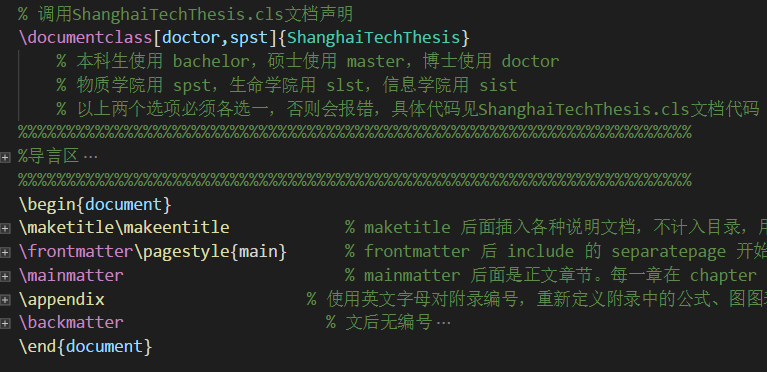
\includegraphics{picture/tex.png}
\section{.cls 文档类的基本结构}
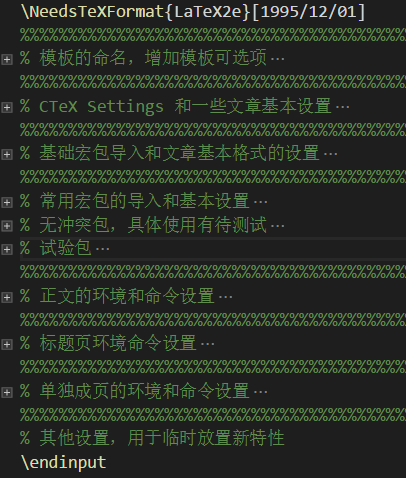
\includegraphics{picture/cls.png}
\section{模板使用方法}
\begin{verbatim}
        1. \documentclass[master,spst]{ShanghaiTechThesis}
        % 本科生使用 bachelor,硕士使用 master,博士使用 doctor
        % 物质学院用 spst,生命学院用 slst,信息学院用 sist
        % 以上两个选项必须各选一,否则会报错,具体见 ShanghaiTechThesis.cls 文档代码

        2. 在 mainmatter 文件夹里按顺序编写论文,如需导入新的宏包或设置新命令,在 .cls 文件设置
        文件引用的文献在 bibliography 文件夹里的 .bib 文件里编译
        文件引用的图片放在 picture 里,用 \includegraphics[]{picture/pic name} 调用
\end{verbatim}
    \chapter{版本使用说明}
\section*{v1.0}
\begin{verbatim}
以 sslchi 前辈在 git@github.com:sslchi/SISTThesis 上的上科大信院毕业论文为基础模板,
参考上海交通大学学位论文模板 SJTUThesis ,进行一系列改进。
    1. 按类别重新整理所有文件的位置
    1. 重新编排.cls 文档的结构,具体结构见 模板使用说明.txt 文档
    2. 为文档类增加所在院系的选项
    3. 修复上科大 logo.png 左下的缺口
    4. 修复用 xelatex 编排时,页眉页脚页码和参考文献无法正确编译的 bug
    5. 修复空白页有页眉页脚 bug
    6. 原创性声明和授权书单独成页
    7. 增加文章结构--算法目录
    8. 增加文章结构--主要符号对照表
    9. 增加文章结构--附录
    10.预定义增加大量宏包,并对部分宏包重新设置
\end{verbatim}

\section*{v1.01}
\begin{verbatim}
    1. 修复算法索引为中文
    2. 模板说明文档小幅更改
    3. 现在能输入长标题了,不过需自行断行。
       取消换行或增加换行,需同时修该 .tex 导言区和 .cls 标题页设置
    4. 增加提交日期中英文的默认选项
    5. 原创性声明和授权声明标题小改
\end{verbatim}

\section*{v1.02}
\begin{verbatim}
    1. 重新编排顺序文件夹
    2. 说明类文档并入 pdf
    3. 修复导言区输入后无法编译bug
    4. 重新编排 .cls文档顺序
\end{verbatim}
    \chapter{bib test}
\section{section}
\subsection{subsection}
\subsubsection{subsubsection}
文献测试一\cite{xiu2010numerical}\\
文献测试二\cite{li2006numerical}\\
文献引用测试三\cite{xia2009real}\\
文献引用测试四\cite{xiu2002wiener}\\
upgreek包测试$\upalpha$


\chapter{文献引用测试2}
\section{节}
\subsection{小节}
\subsubsection{小小节}
文献测试一\cite{xiu2010numerical}\\
文献测试二\cite{li2006numerical}\\
文献引用测试三\cite{xia2009real}\\
文献引用测试四\cite{xiu2002wiener}\\
upgreek包测试$\upalpha$
\appendix	                  % 使用英文字母对附录编号,重新定义附录中的公式、图图表编号样式
    \renewcommand\theequation{\Alph{chapter}--\arabic{equation}}	
    \renewcommand\thefigure{\Alph{chapter}--\arabic{figure}}
    \renewcommand\thetable{\Alph{chapter}--\arabic{table}}
    \renewcommand\thealgorithm{\Alph{chapter}--\arabic{algorithm}}
    \renewcommand\thelstlisting{\Alph{chapter}--\arabic{lstlisting}}
    %% 附录内容,本科学位论文可以用翻译的文献替代。
    \chapter{测试}
附录测试\cite{xia2009real}


\backmatter                     % 文后无编号
    \bibliographystyle{plain}\bibliography{bibliography/book,bibliography/journal} % 生成文献

    % 致谢、发表论文、申请专利、参与项目、简历等, 用于盲审的论文需隐去致谢、发表论文、申请专利、参与的项目
    % 用于盲审的论文需隐去致谢、发表论文、申请专利、参与的项目
    % "研究生学位论文送盲审印刷格式的统一要求" http://www.gs.sjtu.edu.cn/inform/3/2015/20151120_123928_738.htm
    \chapter{致谢}

\vskip 18pt

谨以此文献给所有帮助过我的人。

    % publication 环境具体设置见 .cls 文档 “单独成页的环境和命令设置”
\begin{publications}{99}
\item  {\bf G. Wang} and Q. Liao.``Efficient multi-element spectral stochastic finite element methods for Helmholtz problems close to resonance", about finished.
\item  Q. Liao, D. Silvester and {\bf G. Wang\footnote[1]{Corresponding author.}}. ``Efficient spectral stochastic finite element methods for Helmholtz equations with random inputs'', submitted.
\item J. Zhu and {\bf G. Wang}. ``Fast computation of wave propagation in the open acoustical waveguide with a curved interface",  {\em Wave motion}, {\bf 57}, 171-181, 2015.
\item J. Zhu and {\bf G. Wang}. ``New computational treatment of optical wave propagation in lossy waveguides'',  {\em Frontiers of Information Technology \& Electronic Engineering}, {\bf 16}(8), 646-653, 2015.
\item  J. Zhu and {\bf G. Wang}. ``High-precision computation of optical propagation in gradient refractive-index waveguides'',  {\em Journal of the Optical Society of America A}, {\bf 32}(9), 1653-1660, 2015.
\end{publications}
    % resumesection 和 resumelist 环境设置见 .cls 文件中 “单独成页的环境和命令设置”
\chapter{简\quad 历}

\begin{resumesection}{基本情况}
王官杰,男,浙江大学数学系博士研究生。
\end{resumesection}

\begin{resumelist}{教育状况}
2010 年~9 月至~2015 年~7
月,浙江大学数学系,研究生,专业:计算数学
 
2006 年~9 月至~2010 年~7 月,曲阜师范大学数学科学学院,
本科,专业:数学与应用数学。
\end{resumelist}

\begin{resumelist}{工作经历}
无。
\end{resumelist}

\begin{resumelist}{研究兴趣}
微分方程数值解,计算海洋声学。
\end{resumelist}

\begin{resumelist}{联系方式}
通讯地址:浙江大学数学系 \ \ 邮编:310027

E-mail: wangguanjie0@126.com
\end{resumelist}




\end{document}

